%!TEX program = xelatex
% 完整编译: xelatex -> bibtex -> xelatex -> xelatex
\documentclass[lang=cn,11pt,a4paper,cite=authoryear]{elegantpaper}

\title{Re-Tiling and PPS}
\author{李虎森}

\date{}

% 本文档命令
\usepackage{array}
\newcommand{\ccr}[1]{\makecell{{\color{#1}\rule{1cm}{1cm}}}}

\begin{document}

\maketitle

\begin{abstract}
\\

%本文介绍了一种基于三维点云,重新三角化网格的方法。这种三角化方法有两个实际的应用:
%(1)优化根据Re-Tiling方法[1],生成的网格的缺陷,优化方法正文详细介绍。
本文介绍了一种网格重新三角化的方法,该方法基于Re-Tiling方法[1],但在每个新加入点
确定最终的坐标时,利用网格生成的一种流形曲面,进行了调整,让得到的三角网格更加合理。
%(2)根据三维点云,生成三维网格,这在三维扫描得到点云,转化为网格时比较有用。


\keywords{网格三角化,Re-Tiling,流形曲面}
\end{abstract}


\section{引言}

论文在第二节,简单介绍了Re-Tiling方法[1],并提出了该方法的不足之处。为了做进一步改进,
在第三节,引进了一种根据网格计算光滑流行曲面的一种方法,简记为PPS方法[2]。
第四节根据Re-Tiling和PPS两种方法,对一些网格进行了测试。
% 第五节,介绍了根据三维点云,如何构建出三维网格的方法。
第五节,对方法做了一个小结。

\section{网格重新三角化——Re-Tiling}

该方法的主要目的是,根据输入的原始网格,生成出新的网格,新网格的拓扑结构和原始网格相同,
顶点数和三角面片数增多或者变少,让原始网格变得更加稀疏或者稠密。

主要的思路是,先在网格上(即三角形内部)随机插入$n$(目标定点个数)个顶点,
将插入点和原始网格顶点一起,重新三角化。然后计算每个顶点所收到来自其他插入点的“排斥力”,
排斥力的大小和“排斥半径”$r$有关,当插入点之间距离大于$r$时,排斥力为零。
随后每个插入点根据所受的排斥力,在原始网格上移动。接着重复计算排斥力、
在网格上移动,直到达到迭代次数。
最后,移除原始顶点(能否移除有相应判别准则),并且将顶点的邻域多边形,重新三角化。
这样得到一个新的网格。关于如何在网格上随机插入$n$个点,“排斥力”的计算
和移除原始顶点时的判别准则等详细内容,参见文献[1].

下面介绍Re-Tiling算法流程:\\

输入:封闭的三角网格,目标顶点个数 $n$,排斥力半径$r$。

(1)在网格上随机插入$n$个顶点;

(2)计算每个插入点之间的排斥力;

(3)根据每个插入点所收到的排斥力,将其在原始网格上移动;

(4)循环步骤(2)(3)达到迭代次数;

(5)移除原始顶点。

输出:顶点数为$n$的新网格,拓扑结构与原始网格相同。


\section{Re-Tiling算法优化}
\subsection{Re-Tiling算法不足}
通过第二节的算法步骤,我们可以看到,插入的新顶点只在原始网格上移动,
所以当算法第四步结束时,如果有一个原始三角形上超过三个点,
那么就出现下面这样的情形:

\begin{figure}[!htb]
\centering
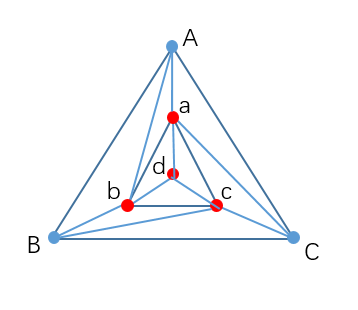
\includegraphics[width=0.3\textwidth]{fig1.png}
\caption{}
\end{figure}

图中A,B,C是原网格上的点,a,b,c,d是插入的点。此时由于a,b,c,d在同一个平面,
这样的点是我们不希望的。

所以下面介绍一种给a,b,c,d找一个新的空间坐标,
让他们即不在同一个平面,又能体现原始网格的形状。
而新的位置将在,由网格生成的流形曲面上去找,这种流形曲面记做PPS[2]。
下面简单介绍PPS的构造,具体构造流程可以参考文献[2]。

\subsection{PPS流形面构造}

PPS流形面,由初始网格生成,它近似于三维网格曲面,与网格曲面的拓扑结构和三维形状是接近的,
区别在于PPS流形是有一定光滑性的曲面。下面来介绍如何根据空间网格构造对应的PPS流形。

流形,顾名思义是由多个同胚于欧式空间的“区域”组成,即由多个类似于$(U,\varphi)$多个$chart$确定,
其中,$U$是流形上“区域”,$\varphi(U)\in \mathbb{R}^n$,为方便我们称之为欧式参数域,设为$V$。
所以在构建PPS流形时,需要先明确
组成流形曲面的“区域”$U$,以及与它们同胚的欧式参数域$V$。

在构建PPS流形时,每个顶点对应一个参数域,
参数域是欧式空间$\mathbb{R}^2$上半径为$|cos(\pi/m_u)|$的圆,
所以,只要确定了光滑映射$\varphi^{-1}$,
那么我们的流形曲面就可以由${\varphi^{-1}(V)}$组成。
$$\varphi^{-1}(p) = \theta_{u}(p)=\sum_{v \in J_{u}(p)} \omega_{v u}(p) 
\times\left(\psi_{v} \circ \varphi_{v u}(p)\right) \quad \quad (*)$$
其中,$p \in V = \Omega_{u}$。这里$\varphi^{-1}$具体构造参见文献[2]。
% 需要注意的是,在计算$\varphi^{-1}(p)$时,只需要直到$p$在$ \Omega_{u}$上的对应的

\section{Re-Tiling 和 PPS}

这一节将具体介绍,怎么将利用PPS优化Re-Tiling算法。

\subsection{Re-Tiling优化}
首先执行Re-Tiling算法流程的步骤(1)——(4),在移除原始顶点之前,将插入点对应到参数域$V$上,
然后利用3.2中公式(*),计算出每个插入点对应到PPS流形中的坐标,
将PPS流形上的坐标作为每个插入点的新坐标,这样由于流形曲面的光滑性和表面凹凸性,
每个插入点就可以有一个更合理的空间坐标,就能较好的避免“四点共面”的情形。

\subsection{效果展示}

\begin{figure}[!htb]
\centering
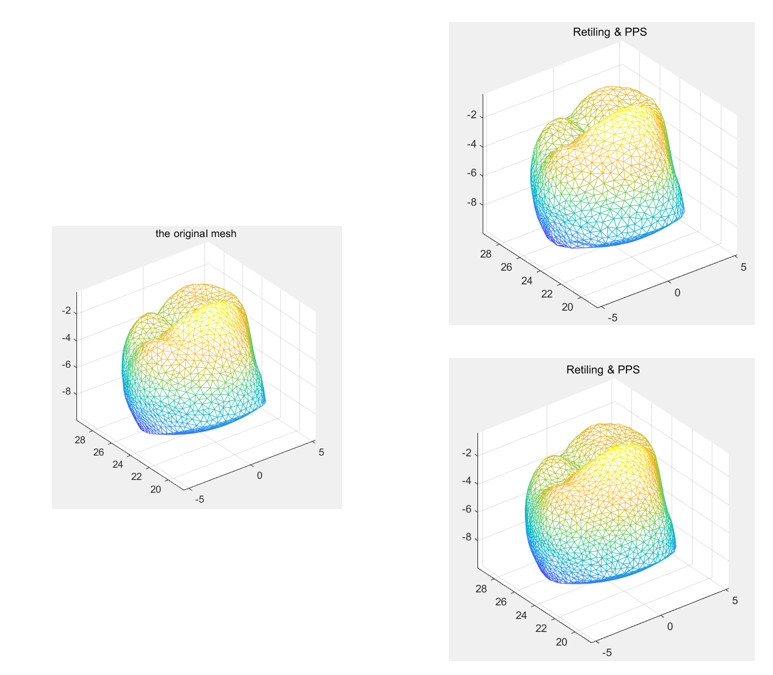
\includegraphics[width=0.8\textwidth]{fig2.png}
\caption{}
\end{figure}

\begin{figure}[!htb]
\centering
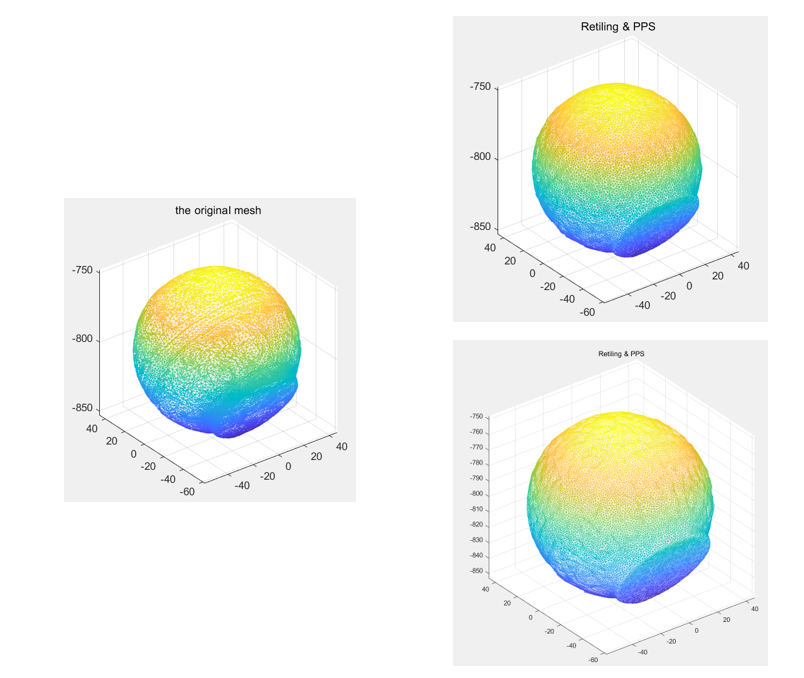
\includegraphics[width=0.8\textwidth]{fig3.png}
\caption{}
\end{figure}


\begin{center}
\begin{tabular}{cccccc}
\toprule  %添加表格头部粗线
模型名称& 顶点数& 面数& 目标顶点数& 目标面数& 耗时(单位:秒)\\
\midrule  %添加表格中横线
1&	1967&	3930&	   1458&	2912&	17s\\
 &      &     &    2424&	4844&	19s\\

\midrule %\hline
2& 19483&  38962&  14666&	  29328&	  222s\\
 &	     &	    &	24369&	48788&	261s\\

\bottomrule %添加表格底部粗线
\end{tabular}
\end{center}




\section{小结}
点云到网格

在点云生成网格前,我们需要有一个初始网格,这个初始网格代表了点云所表示的物体的拓扑结构。
下面是我们算法的流程:

Re-Tiling and PPS

输入:封闭的三角网格,目标顶点个数 $n$,排斥力半径$r$。

(1)在网格上随机插入$n$个顶点;

(2)计算每个插入点之间的排斥力;

(3)根据每个插入点所收到的排斥力,将其在原始网格上移动;

(4)循环步骤(2)(3)达到迭代次数;

(5)计算出插入点在PPS流形上的位置,流形上的位置,更新现在的位置。

(6)移除原始顶点。

输出:顶点数为$n$的新网格,拓扑结构与原始网格相同。


\section{参考文献}
[1].Greg Turk, Re-Tiling Polygonal Surfaces.

[2].Marcelo Siqueira, Dianna Xu,A new construction of smooth surfaces 
from triangle meshes using parametric pseudo-manifolds.
\end{document}
